\documentclass[11pt]{article}
% \usepackage{lipsum} % not available on dreamhost
\usepackage{charsheet}
\usepackage{multicol}

\usepackage{pgfkeys}

% Incomplete character support
\newif\ifcomplete
\completetrue  % Default to complete character



\newsectionenv[]{magic}{MAGIC}
  {\begin{minipage}[t]{\hsize}
   \featurespostspace=0pt
   \useDNDfont{MAGIC}
  }
  {\end{minipage}}
\newsectionenv{attacks}{ATTACKS}{}{}
\newsectionenv{features}{FEATURES}{}{}
\newsectionenv[width=70mm,decorated clipped rectangle]{equipment}{EQUIPMENT}
   {\medskip
    \ifDNDdefined{MAGIC}{}{\begin{multicols}{2}}%
    \small
     \begin{eqlist}}
   {\end{eqlist}%
    \ifDNDdefined{MAGIC}{}{\end{multicols}}%
   }


\newsectionenv[width=38mm]{proficiencies}{PROFICIENCIES}
   {\medskip
    \begin{minipage}[t][138mm][t]{\hsize}
     \begin{proflist}}
   {\end{proflist}
    \end{minipage}}

  

\begin{document}


\newcommand\nextstatloc{inside north west corner=of stats background}



%\makeatletter
%\newcommand{\stat@starred}[2]{%
%  \newcounter{tempmodifier}%
%  \newcounter{tempmodifierwithprof}%
%  \setcounter{tempmodifier}{(#2 - 10) / 2}%
%  \setcounter{tempmodifierwithprof}{\value{tempmodifier} + \value{proficiencybonus}}%
%  \fullstatbox[\nextstatloc]{#1}{#2}{\thetempmodifier}{\thetempmodifierwithprof}%
%}
%\newcommand{\stat@}{\@ifstar{\stat@starred}{\stat}}
%\let\stat\stat@
%\makeatother


\noindent
\begin{charsheet}

\input{zanogh}
%\input{miriel}
%\input{kylane3}
%  \setcounter{proficiency bonus}{2}

  \node [dndfull,height=20mm,fill=playername,below=of top] (splash) 
     {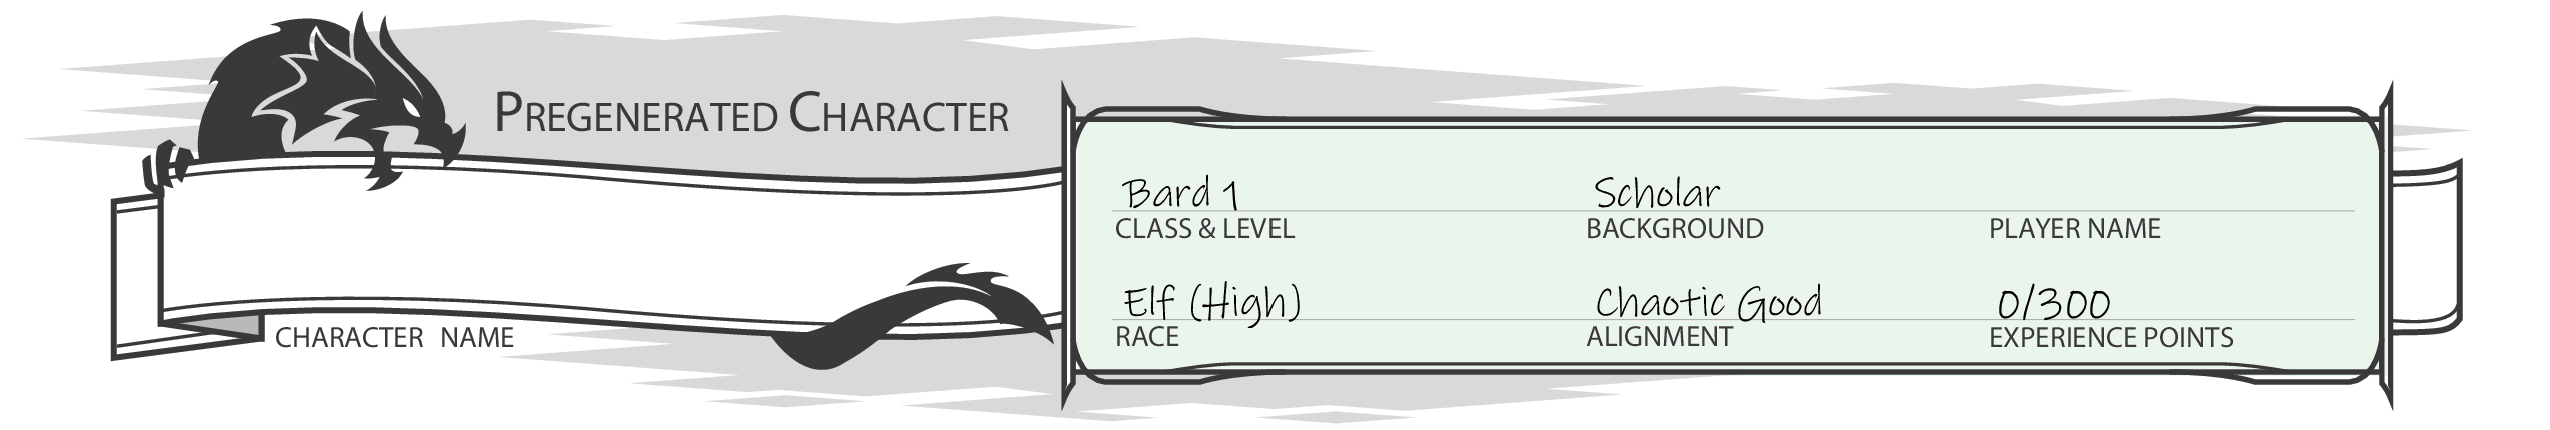
\includegraphics[width=\textwidth]{splash.png}};

  \colorlet{splashgray}{white!85.765!black}



  \begingroup\sffamily

  \newcommand\namestrut{\vrule width 0pt depth 1pt\relax}

  \path ($(splash.south west)+(88mm,18.75mm)$) coordinate  (class field sw);
  \path ($(splash.south west)+(88mm,9.7mm)$) coordinate  (race field sw);
  \path ($(splash.south west)+(48mm,16mm)$) coordinate  (charname center);
  \path ($(splash.south west)+(40mm,24mm)$) coordinate  (pregen left);
 

  \ifDNDfalse{PREGENERATED}%
    {\node [fill=splashgray,width=42mm,height=5mm,anchor=south west,at=(pregen left)] {};}
    {}


  \node [fill=splashfield,width=97mm,height=6mm,anchor=south west,at=(class field sw)] {};
  \node [fill=splashfield,width=97mm,height=6mm,anchor=south west,at=(race field sw)] {};

  \path (class field sw) +(0mm,0.6mm) coordinate (class sw);
  \path (race field sw) +(0mm,0.6mm) coordinate (race sw);

  \writesplash[at=(class sw)]{34mm}{CLASS + LEVEL}
  \writesplash[right of base=1mm of CLASS + LEVEL]{28mm}{BACKGROUND}
  \writesplash[right of base=1mm of BACKGROUND]{34mm}{PLAYER NAME}

  \writesplash[at=(race sw)]{34mm}{RACE}
  \writesplash[right of base=1mm of RACE]{34mm}{ALIGNMENT}
  \writesplash[right of base=1mm of ALIGNMENT]{34mm}{EXPERIENCE POINTS}

  \ifDNDdefined{CHARACTER NAME}
{\node[at=(charname center),font={\rmfamily\LARGE\itshape},anchor=center]
      {\getDND{CHARACTER NAME}\ifDNDnonempty{AGE}{ (\getDND{AGE})}{}}
      ;
    }
    {}

\Large

      \node (hpbackground) 
        [outer sep=0pt,fill=hpetc,below right corner=of splash,width=102mm, minimum height=46mm] 
       { };

      \node (hitdice)
             [dndhits,width=20mm,inside south east corner=of hpbackground,
             dndlabel=HIT DICE] 
         { \Large \getDND*{HIT DICE}{} }
         ;

     \ifDNDdefined{LEVEL}{
         \node [at=(hitdice.north),anchor=north] 
              {\expandafter\stackslots\expandafter{\rawgetDND{LEVEL}+1}};
     }{}

      \node (curhp)
            [dndhits,fill=white,width=72mm,left=of hitdice,
             dnd/label={CURRENT HIT POINTS}] 
         { }
         ;

      \node [dndmaxhp,above left corner=of curhp,dndlabel=MAX HP] 
         (maxhp)
         { \Large \getDND*{MAX HP} }
         ;

      \node (initiative)
            [dndmaxhp,right=of maxhp,dndlabel=INITIATIVE] 
         { \getDND*{INITIATIVE} }
         ;

%\node [draw,above=of initiative] % {\slotsliteral7};
%              {\expandafter\stackslots\expandafter{\rawgetDND{LEVEL}+1}};


      \node (speed)
            [dndmaxhp,right=of initiative,dndlabel=SPEED] 
         { \getDND*{SPEED} }
         ;


       \node (ac) [dndmaxhp,shield,innershield,draw,ultra thick,right=of speed,width=15mm,
                   dndlabel={\noexpand\tinystacklabel{ARMOR}{CLASS}},
            ]
      {\raisebox{4mm}{\getDND*{ARMOR CLASS}}}
      ;

  \endgroup


\begin{attacks}[below right corner=of hpbackground]{}
    \centering
    \begin{attackstab}
    \getDND{ATTACKS}
    \end{attackstab}
\end{attacks}


% \node (attacks) at (hpbackground.south west) {A};

\ifDNDdefined{MAGIC}
{
\begin{magic}[below=of attacks]{}
\centering
\begin{featurestab}
% Magic section (right side, middle)
\rawgetDND{MAGIC}
%  \textsf{CANTRIPS}\\
%  Friends& Does a thing\\
%  Ray of Frost& asdf\\
%  \multicolumn2{l}{\textsf{1st-LEVEL SPELLS \spellslots{3}}}\\
\end{featurestab}
\end{magic}
}
{\path (attacks.south east) coordinate (magic);} % anchor is to east

\ifDNDdefined{FEATURES}{
  \ifDNDdefined{MAGIC}
     {\def\where{anchor=south east,at=(current bounding box.south -| magic.east)}}
     {\def\where{below right corner=of attacks}}%
  \beginExpand{features}[\where]{}
  \let\described=\feature
  \begin{featurestab}
  \getDND{FEATURES}
  \end{featurestab}
  \end{features}
}{}

\node (stats background) 
      [fill=stats,width=24mm,height=163mm,below left corner=of splash] { };

\newcommand{\incompletestat}[2]{% label, short name
  \ifDNDnonempty{#2}{%
    \dndstat{#1}{#2}%
  }{%
    \expandafter\blankstatbox\expandafter[\nextstatloc]{#1}
             {\ifDNDnonempty{#2 SAVING}{*}{}}%
    \gdef\nextstatloc{below=7mm of #1}%
  }%
}

\ifcomplete
  \dndstat{STRENGTH}{STR}
  \dndstat{DEXTERITY}{DEX}
  \dndstat{CONSTITUTION}{CON}
  \dndstat{INTELLIGENCE}{INT}
  \dndstat{WISDOM}{WIS}
  \dndstat{CHARISMA}{CHA}
\else
  \incompletestat{STRENGTH}{STR}
  \incompletestat{DEXTERITY}{DEX}
  \incompletestat{CONSTITUTION}{CON}
  \incompletestat{INTELLIGENCE}{INT}
  \incompletestat{WISDOM}{WIS}
  \incompletestat{CHARISMA}{CHA}
\fi

% slots OK here

\typeout{WTF magic}
  
\ifDNDdefined{EQUIPMENT}{%
%  \typeout{equipment, not magic}%
  {%
   \ifDNDdefined{MAGIC}{\def\where{left of lower corner=of features}}
                       {\def\where{below right corner=of features,width=\dndrightwidth}}%

  \beginExpand{equipment}[\where]
     \useDNDfont{EQUIPMENT}%
     \getDND{EQUIPMENT}
  \end{equipment}
  }
}
{\node (equipment) [left of lower corner=of features] {};
}

\path (equipment.north west) +(3mm,-4mm) coordinate (coin top left);


\coin{cp}{Cu}{\getDND*{CP}}
\coin{sp}{Ag}{\getDND*{SP}}
\coin{gp}{Au}{\getDND*{GP}}
  
\node (proficiency bonus)
      [proficiencies,decorated stub rectangle,width=38.001mm,height=8mm,
       right of upper corner=3.5mm of stats background]
   {\hbox to 0pt{\hss\hspace*{9mm}\tiny\textsf{PROFICIENCY BONUS}\hss}}
   ;
\node [anchor=west,proficiencies,circle,
       width=10mm,height=10mm,line width=1.5pt,draw]
       at ($(proficiency bonus.west)+(-2mm,0mm)$)
      {\large\textsf{+\arabic{proficiency bonus}}};

% Proficiencies section (middle top)
\begin{proficiencies}[below=of proficiency bonus,width=38.002mm,height=3in]
  \small
\getDND*{PROFICIENCIES}
\end{proficiencies}

%\node (motivation) [below=of proficiencies] 
%  {\parbox{36mm}{\Large\centering\textit{\getDND*{MOTIVATION}}}}
%  ;

\node (motivations) [above=4.45mm of BACKGROUND.north] 
  {\Large\textit{\getDND*{MOTIVATION}}}
  ;


%\node [draw,below=of initiative] % {\slotsliteral7};
%              {\expandafter\stackslots\expandafter{\rawgetDND{LEVEL}+5}};


\firsttwoDNDnonempty{\upperdndlabel}{\upperdndcontents}{\lowerdndlabel}{\lowerdndcontents}{SORCERY POINTS,SENSES,SPELL DC,PASSIVE PERCEPTION}

%\typeout{upper is \upperdndlabel; lower is \lowerdndlabel}

%{\ifDNDnonempty{SENSES}{\typeout{SENSES IS NOT EMPTY; it is !\rawgetDND{SENSES}!}}{}}

%\node [draw,below=of maxhp] % {\slotsliteral7};
%              {\expandafter\stackslots\expandafter{\rawgetDND{LEVEL}+1}};

% slots not OK here


%\ifDNDdefined{SPELL DC}
%  {
%      \node (spell dc)
%         [dndmaxhp,left=10mm of maxhp,width=24mm] 
%         {\Large\textsf{13}}
%         ;
%
%      \dndlabel{spell dc}{SPELL DC}
%  }
%  {
%      \node (passive perception)
%         [dndmaxhp,left=10mm of maxhp,width=24mm] 
%         {\Large\textsf{\getDND*{PASSIVE PERCEPTION}}}
%         ;
%
%      \dndlabel{passive perception}{\pplabel}
%  }
%
%\node (senses)
%   [dndmaxhp,left=10mm of curhp,width=24mm] 
%%   {\itshape\begin{tabular}{c}{Darkvision}\\{60~ft}\\[3pt]\end{tabular}}
%   {\parbox{20mm}{\centering\itshape\getDND*{SENSES}}}
%   ;
%\dndlabel{senses}{\scriptsize SENSES}
%
%

\def\sp{SORCERY POINTS}
\ifx\upperdndlabel\sp
  \edef\upperdndcontents{\noexpand\stackslots{\rawgetDND{SORCERY POINTS}}}%
\fi

\def\se{SENSES}
\ifx\upperdndlabel\se
  \def\upperdndcontents{\parbox{20mm}{\centering\rmfamily\small\textit{\getDND{SENSES}}}}%
\fi

%\show\pp
%\show\upperdndlabel

  \node (upper val)
         [dndmaxhp,left=10mm of maxhp,width=24mm] 
         {\Large\textsf{\upperdndcontents}}
         ;

      \ifDNDfont{\upperdndlabel}
         {\dndlabel[\upperdndlabel]{upper val}{\upperdndlabel}}
         {\dndlabel{upper val}{\upperdndlabel}}

\ifx\lowerdndlabel\empty\else

   \node (lower val)
      [dndmaxhp,left=10mm of curhp,width=24mm] 
      {\Large\textsf{\lowerdndcontents}}
      ;
      \ifDNDfont{\lowerdndlabel}
         {\dndlabel[\lowerdndlabel]{lower val}{\lowerdndlabel}}
         {\dndlabel{lower val}{\lowerdndlabel}}

\fi


%\node [draw,above=of features] {\parbox{4in}{7 slots: minimum \minrows{7} rows\par \stackslots7\par\hbox{\slotsliteral3}}};


\end{charsheet}

% Equipment Weight Summary Page
\clearpage

\begin{charsheet}
\input{stats}

% Define colors for capacity boxes
\colorlet{carryingcolor}{white}
\colorlet{encumberedcolor}{proficiencies}  % Use existing yellow from charsheet.sty
\colorlet{heavilyencumberedcolor}{magic}   % Use existing red from charsheet.sty

% Define height per tenth of stone for equipment slots
\newdimen\tenthstoneheight
\tenthstoneheight=8pt

% Calculate total weight (in tenths of stones)
\newcounter{totalWeight}
\setcounter{totalWeight}{\value{weightHeavyWeapons}}
\addtocounter{totalWeight}{\value{weightNormalWeapons}}
\addtocounter{totalWeight}{\value{weightLightWeapons}}
\addtocounter{totalWeight}{\value{weightShields}}
\addtocounter{totalWeight}{\value{weightHeavyArmor}}
\addtocounter{totalWeight}{\value{weightNormalArmor}}
\addtocounter{totalWeight}{\value{weightLightArmor}}
\addtocounter{totalWeight}{\value{weightHeavyItems}}
\addtocounter{totalWeight}{\value{weightSlottedItems}}
\addtocounter{totalWeight}{\value{weightFreeItems}}

% Calculate carrying capacity thresholds (in tenths of stones)
\newcounter{carryingCapacity}
\newcounter{encumberedThreshold}
\newcounter{heavilyEncumberedThreshold}

\ifDNDnonempty{STR}{%
  % Carrying capacity = STR score in stones (convert to tenths)
  \setcounter{carryingCapacity}{\numexpr\rawgetDND{STR} * 10\relax}
  
  % Encumbered = 1/3 of carrying capacity, rounded down
  \setcounter{encumberedThreshold}{\numexpr\rawgetDND{STR} * 10 / 3\relax}
  
  % Heavily encumbered = 2/3 of carrying capacity, rounded down  
  \setcounter{heavilyEncumberedThreshold}{\numexpr\rawgetDND{STR} * 20 / 3\relax}
}{%
  % No STR defined - leave counters at zero
}

% Three capacity boxes centered below top
\node (encumbered) [dndencumbrance,fill=encumberedcolor,below=of top,dndlabel=ENCUMBERED] 
  {\Large\ifDNDnonempty{STR}{\textbf{$\geq$ \renderstones{\arabic{encumberedThreshold}}}}{empty
  STR?}};

\node (carrying) [dndencumbrance,fill=carryingcolor,left=5mm of encumbered,dndlabel=CARRYING CAPACITY]
  {\Large\ifDNDnonempty{STR}{\textbf{$\leq$ \renderstones{\arabic{carryingCapacity}}}}{}};

\node (heavily) [dndencumbrance,fill=heavilyencumberedcolor,right=5mm of encumbered,dndlabel=HEAVILY ENCUMBERED]
  {\Large\ifDNDnonempty{STR}{\textbf{$\geq$ \renderstones{\arabic{heavilyEncumberedThreshold}}}}{}};

% Calculate remaining capacity for light weapons and slotted items (in stones)
\newcounter{significantWeight}
\setcounter{significantWeight}{\value{weightHeavyWeapons}}
\addtocounter{significantWeight}{\value{weightNormalWeapons}}
\addtocounter{significantWeight}{\value{weightShields}}
\addtocounter{significantWeight}{\value{weightHeavyArmor}}
\addtocounter{significantWeight}{\value{weightNormalArmor}}
\addtocounter{significantWeight}{\value{weightLightArmor}}
\addtocounter{significantWeight}{\value{weightHeavyItems}}

\newcounter{remainingCapacity}
\ifDNDnonempty{STR}{%
  % Remaining = carrying capacity - significant weight (in tenths of stones)
  \setcounter{remainingCapacity}{\numexpr\rawgetDND{STR} * 10 - \value{significantWeight}\relax}
  % Convert to stones and multiply by 5 for line count
  \setcounter{remainingCapacity}{\numexpr\value{remainingCapacity} * 5 / 10\relax}
}{%
  \setcounter{remainingCapacity}{0}
}

% Equipment slots box on the left with three-color backgrounds
% First calculate positions for color transitions in terms of \tenthstoneheight
\newcounter{greenLines}
\newcounter{yellowLines}  
\newcounter{redLines}

\ifDNDnonempty{STR}{%
  % Calculate how many lines each color region should have
  % Total lines = 5 * remaining capacity (in stones)
  \setcounter{greenLines}{\numexpr\value{encumberedThreshold} * 5 / 10\relax}%
  \setcounter{yellowLines}{\numexpr(\value{heavilyEncumberedThreshold} - \value{encumberedThreshold}) * 5 / 10\relax}%
  \setcounter{redLines}{\numexpr(\value{carryingCapacity} - \value{heavilyEncumberedThreshold}) * 5 / 10\relax}%
}{%
  \setcounter{greenLines}{0}%
  \setcounter{yellowLines}{0}%
  \setcounter{redLines}{0}%
}

% Calculate heights for each color region
\newdimen\greenheight
\newdimen\yellowheight
\newdimen\redheight

\greenheight=\numexpr\value{greenLines}\relax\tenthstoneheight
\yellowheight=\numexpr\value{yellowLines}\relax\tenthstoneheight  
\redheight=\numexpr\value{redLines}\relax\tenthstoneheight

% Create the equipment slots box with colored backgrounds
\node (slots) [dndbox,minimum width=60mm,minimum height=\dimexpr\greenheight+\yellowheight+\redheight+10mm\relax,right=of current bounding box.west,anchor=west] {
  \begin{tabular}{l}
  \toprule
  \textbf{Equipment slots} \\
  \midrule
  % Add light weapons in light gray
  \ifDNDnonempty{LIGHT WEAPONS}{\color{gray}\getDND{LIGHT WEAPONS}}{}%
  % Add slotted items in light gray  
  \ifDNDnonempty{SLOTTED ITEMS}{\color{gray}\getDND{SLOTTED ITEMS}}{}%
  \bottomrule
  \end{tabular}
};

% Add colored background rectangles behind the slots box
\ifnum\value{greenLines}>0\relax
  \fill [green!30] ([yshift=-2mm]slots.north west) rectangle ([yshift=-\greenheight-2mm]slots.north east);
\fi
\ifnum\value{yellowLines}>0\relax  
  \fill [yellow!50] ([yshift=-\greenheight-2mm]slots.north west) rectangle ([yshift=-\greenheight-\yellowheight-2mm]slots.north east);
\fi
\ifnum\value{redLines}>0\relax
  \fill [red!30] ([yshift=-\greenheight-\yellowheight-2mm]slots.north west) rectangle ([yshift=-\greenheight-\yellowheight-\redheight-2mm]slots.north east);
\fi

% Significant equipment list on the right
\node [dndbox,minimum width=60mm,right=10mm of heavily,anchor=north west] {
  \begin{tabular}{lr}
  \toprule
  \emph{Equipment} & \emph{Weight} \\
  \midrule
  % Include all equipment except SLOTTED ITEMS, LIGHT WEAPONS, and FREE ITEMS
  % TODO: Add actual equipment items
  \bottomrule
  \end{tabular}
};

% Equipment weight breakdown table
\node [below=10mm of encumbered,anchor=north] {
  \begin{tabular}{lr}
  \toprule
  \emph{Category} & \emph{Weight (stones)} \\
  \midrule
  % Display non-zero weight categories
  \ifnum\value{weightHeavyWeapons}>0 \relax
  Heavy weapons & \renderstones{\value{weightHeavyWeapons}} \\
  \fi
  \ifnum\value{weightNormalWeapons}>0 \relax
  Normal weapons & \renderstones{\value{weightNormalWeapons}} \\
  \fi
  \ifnum\value{weightLightWeapons}>0 \relax
  Light weapons & \renderstones{\value{weightLightWeapons}} \\
  \fi
  \ifnum\value{weightShields}>0 \relax
  Shields & \renderstones{\value{weightShields}} \\
  \fi
  \ifnum\value{weightHeavyArmor}>0 \relax
  Heavy armor & \renderstones{\value{weightHeavyArmor}} \\
  \fi
  \ifnum\value{weightNormalArmor}>0 \relax
  Normal armor & \renderstones{\value{weightNormalArmor}} \\
  \fi
  \ifnum\value{weightLightArmor}>0 \relax
  Light armor & \renderstones{\value{weightLightArmor}} \\
  \fi
  \ifnum\value{weightHeavyItems}>0 \relax
  Heavy items & \renderstones{\value{weightHeavyItems}} \\
  \fi
  \ifnum\value{weightSlottedItems}>0 \relax
  Slotted items & \renderstones{\value{weightSlottedItems}} \\
  \fi
  \ifnum\value{weightFreeItems}>0 \relax
  Free items & \renderstones{\value{weightFreeItems}} \\
  \fi
  \midrule
  \textbf{Total} & \textbf{\renderstones{\value{totalWeight}}} \\
  \bottomrule
  \end{tabular}
};

\end{charsheet}

\end{document}
